\section*{\centering BAB IV \\ Metode Penelitian}

\addcontentsline{toc}{section}{BAB IV Metode Penelitian}  % Manually add unnumbered section to ToC

% Set the section counter manually to "1" for subsections under BAB IV
\setcounter{section}{4}
\setcounter{subsection}{0}  % Reset subsection
\setcounter{figure}{0}
\renewcommand{\thefigure}{\thesection.\arabic{figure}}

\subsection{Analisis Permasalahan}
KPU Provinsi Lampung saat ini sedang melaksanakan agenda lima tahunan Pilkada. Sebagai bagian dari persiapan Pilkada 2024, KPU Provinsi Lampung telah melakukan rekapitulasi daftar pemilih. Namun, untuk memahami distribusi dan karakteristik daftar pemilih antar kecamatan di 15 Kabupaten Lampung, diperlukan sebuah analisis yang lebih mendalam. Solusi yang diusulkan adalah penerapan teknik klusterisasi pada data rekapitulasi tersebut, serta penggunaan data opsional lain dari BPS untuk memperkaya analisis. Hasil klusterisasi ini diharapkan dapat memberikan wawasan tambahan melalui visualisasi interaktif yang lebih informatif.

\subsection{Alur Penyelesaian}
\begin{figure}[h]
    \centering
    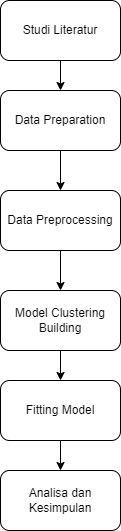
\includegraphics[width=0.2\linewidth, height=10cm]{images/flow.png}
    \caption{Alur Penyelesaian Penelitian}
    \label{fig:flow}
\end{figure}

\subsubsection{Studi Literatur}
Pada tahap ini, penulis melakukan kajian literatur yang berkaitan dengan klusterisasi data, baik pada data pemilih maupun data umum lainnya. Tujuannya adalah untuk memahami atribut-atribut data penting yang akan menjadi basis penelitian ini.

\subsubsection{Data Preparation}
Persiapan data (\textit{data preparation}) adalah tahap awal sebelum data dapat digunakan dalam model. Pada tahap ini, data masih dalam bentuk mentah dan belum melalui proses normalisasi.

\subsubsection{Data Preprocessing}
Setelah data terkumpul, dilakukan tahap praproses data (\textit{data preprocessing}). Pada tahap ini, penulis menentukan atribut yang relevan untuk proses klusterisasi dan melakukan normalisasi data guna memastikan keseragaman skala atribut.

\subsubsection{Model Kluster Building}
Dalam tahap ini, penulis membangun model klusterisasi. Jumlah kluster yang optimal akan ditentukan menggunakan metode \textit{Elbow}, dan model klusterisasi akan dibangun menggunakan algoritma \textit{K-Means}.

\subsubsection{Penerapan Model}
Setelah jumlah kluster yang sesuai telah ditentukan, data akan dimasukkan ke dalam model klusterisasi yang telah dibangun. Visualisasi hasil klusterisasi dari berbagai perspektif akan dilakukan untuk memperoleh wawasan yang lebih baik mengenai rekapitulasi daftar pemilih.

\subsubsection{Analisis dan Kesimpulan}
Tahap ini mencakup analisis hasil klusterisasi dan penyusunan kesimpulan berdasarkan model yang telah dibangun. Penulis juga akan mengevaluasi performa model, mengidentifikasi kelebihan dan kekurangannya, serta menentukan apakah hasil analisis sudah sesuai dengan tujuan awal penelitian.

\subsection{Alat dan Bahan}
Penelitian ini menggunakan \textit{Google Colab} sebagai platform utama untuk membangun model klusterisasi. Data yang digunakan bersumber dari KPU dan BPS sebagai bahan utama dalam penelitian.

\newpage